\documentclass[11pt,a4paper]{letter}\usepackage[]{graphicx}\usepackage[]{color}
%% maxwidth is the original width if it is less than linewidth
%% otherwise use linewidth (to make sure the graphics do not exceed the margin)
\makeatletter
\def\maxwidth{ %
  \ifdim\Gin@nat@width>\linewidth
    \linewidth
  \else
    \Gin@nat@width
  \fi
}
\makeatother

\definecolor{fgcolor}{rgb}{0.345, 0.345, 0.345}
\newcommand{\hlnum}[1]{\textcolor[rgb]{0.686,0.059,0.569}{#1}}%
\newcommand{\hlstr}[1]{\textcolor[rgb]{0.192,0.494,0.8}{#1}}%
\newcommand{\hlcom}[1]{\textcolor[rgb]{0.678,0.584,0.686}{\textit{#1}}}%
\newcommand{\hlopt}[1]{\textcolor[rgb]{0,0,0}{#1}}%
\newcommand{\hlstd}[1]{\textcolor[rgb]{0.345,0.345,0.345}{#1}}%
\newcommand{\hlkwa}[1]{\textcolor[rgb]{0.161,0.373,0.58}{\textbf{#1}}}%
\newcommand{\hlkwb}[1]{\textcolor[rgb]{0.69,0.353,0.396}{#1}}%
\newcommand{\hlkwc}[1]{\textcolor[rgb]{0.333,0.667,0.333}{#1}}%
\newcommand{\hlkwd}[1]{\textcolor[rgb]{0.737,0.353,0.396}{\textbf{#1}}}%
\let\hlipl\hlkwb

\usepackage{framed}
\makeatletter
\newenvironment{kframe}{%
 \def\at@end@of@kframe{}%
 \ifinner\ifhmode%
  \def\at@end@of@kframe{\end{minipage}}%
  \begin{minipage}{\columnwidth}%
 \fi\fi%
 \def\FrameCommand##1{\hskip\@totalleftmargin \hskip-\fboxsep
 \colorbox{shadecolor}{##1}\hskip-\fboxsep
     % There is no \\@totalrightmargin, so:
     \hskip-\linewidth \hskip-\@totalleftmargin \hskip\columnwidth}%
 \MakeFramed {\advance\hsize-\width
   \@totalleftmargin\z@ \linewidth\hsize
   \@setminipage}}%
 {\par\unskip\endMakeFramed%
 \at@end@of@kframe}
\makeatother

\definecolor{shadecolor}{rgb}{.97, .97, .97}
\definecolor{messagecolor}{rgb}{0, 0, 0}
\definecolor{warningcolor}{rgb}{1, 0, 1}
\definecolor{errorcolor}{rgb}{1, 0, 0}
\newenvironment{knitrout}{}{} % an empty environment to be redefined in TeX

\usepackage{alltt}
\usepackage[top=1.00in, bottom=1.0in, left=1.1in, right=1.1in]{geometry}
\usepackage{graphicx}

%\signature{}
\IfFileExists{upquote.sty}{\usepackage{upquote}}{}
\begin{document}
\begin{letter}{}

\includegraphics[width=0.3\textwidth]{AA_logo.jpg}

\opening{Dear Global Change Biology Editorial Office:}

\noindent Please consider our revised manuscript `Rethinking False Spring Risk' as an Opinion for \emph{Global Change Biology.} 
\vspace{1.5ex}\\
Climate change has brought renewed interest to a major factor that shapes the life history of many non-tropical plant species: late spring freeze events, commonly called false springs. While increased interest has led to a growing number of studies, much of the research takes a simplified view of these events, which---we argue---can lead to incorrect estimates and forecasting. Combining theory from ecology, climatology, physiology, biogeography and crop science we examine the effects of false springs, and the complexity of factors that drive plants' risk to frost damage.
\vspace{1.5ex}\\
Comments from three reviewers have greatly improved this manuscript and led us to refine the overall structure, enhance major discussion points, and address future directions to a greater extent. We have added a new section, \textit{The future of false spring research}, and renamed and reframed most other sections. Additionally, we added, adjusted and moved much of the text (including several whole sections) to improve the manuscript's flow and coherency in light of reviewers' comments. To address concerns from all three reviewers regarding floral bud freezing risk, we moved portions of the text to earlier in the manuscript to stress our focus on vegetative phenophases. We also added information to the sections \emph{Measuring false spring in one temperate plant community} for Figure 2 and \emph{Integrating predictable regional differences in false spring risk} for Figure 5 to provide more information about the data and methods we used.
\vspace{1.5ex}\\
We have attempted to address all reviewer concerns and detail our changes in our point-by-point response (note that reviewer comments are in \emph{italics}, while our responses are in regular text). We feel the new submission is much improved. This Opinion piece is not under examination for publication elsewhere. We hope that you will find it suitable for \emph{Global Change Biology}, and look forward to hearing from you.
\\\vspace{-1ex}\\
\noindent Sincerely,\\

 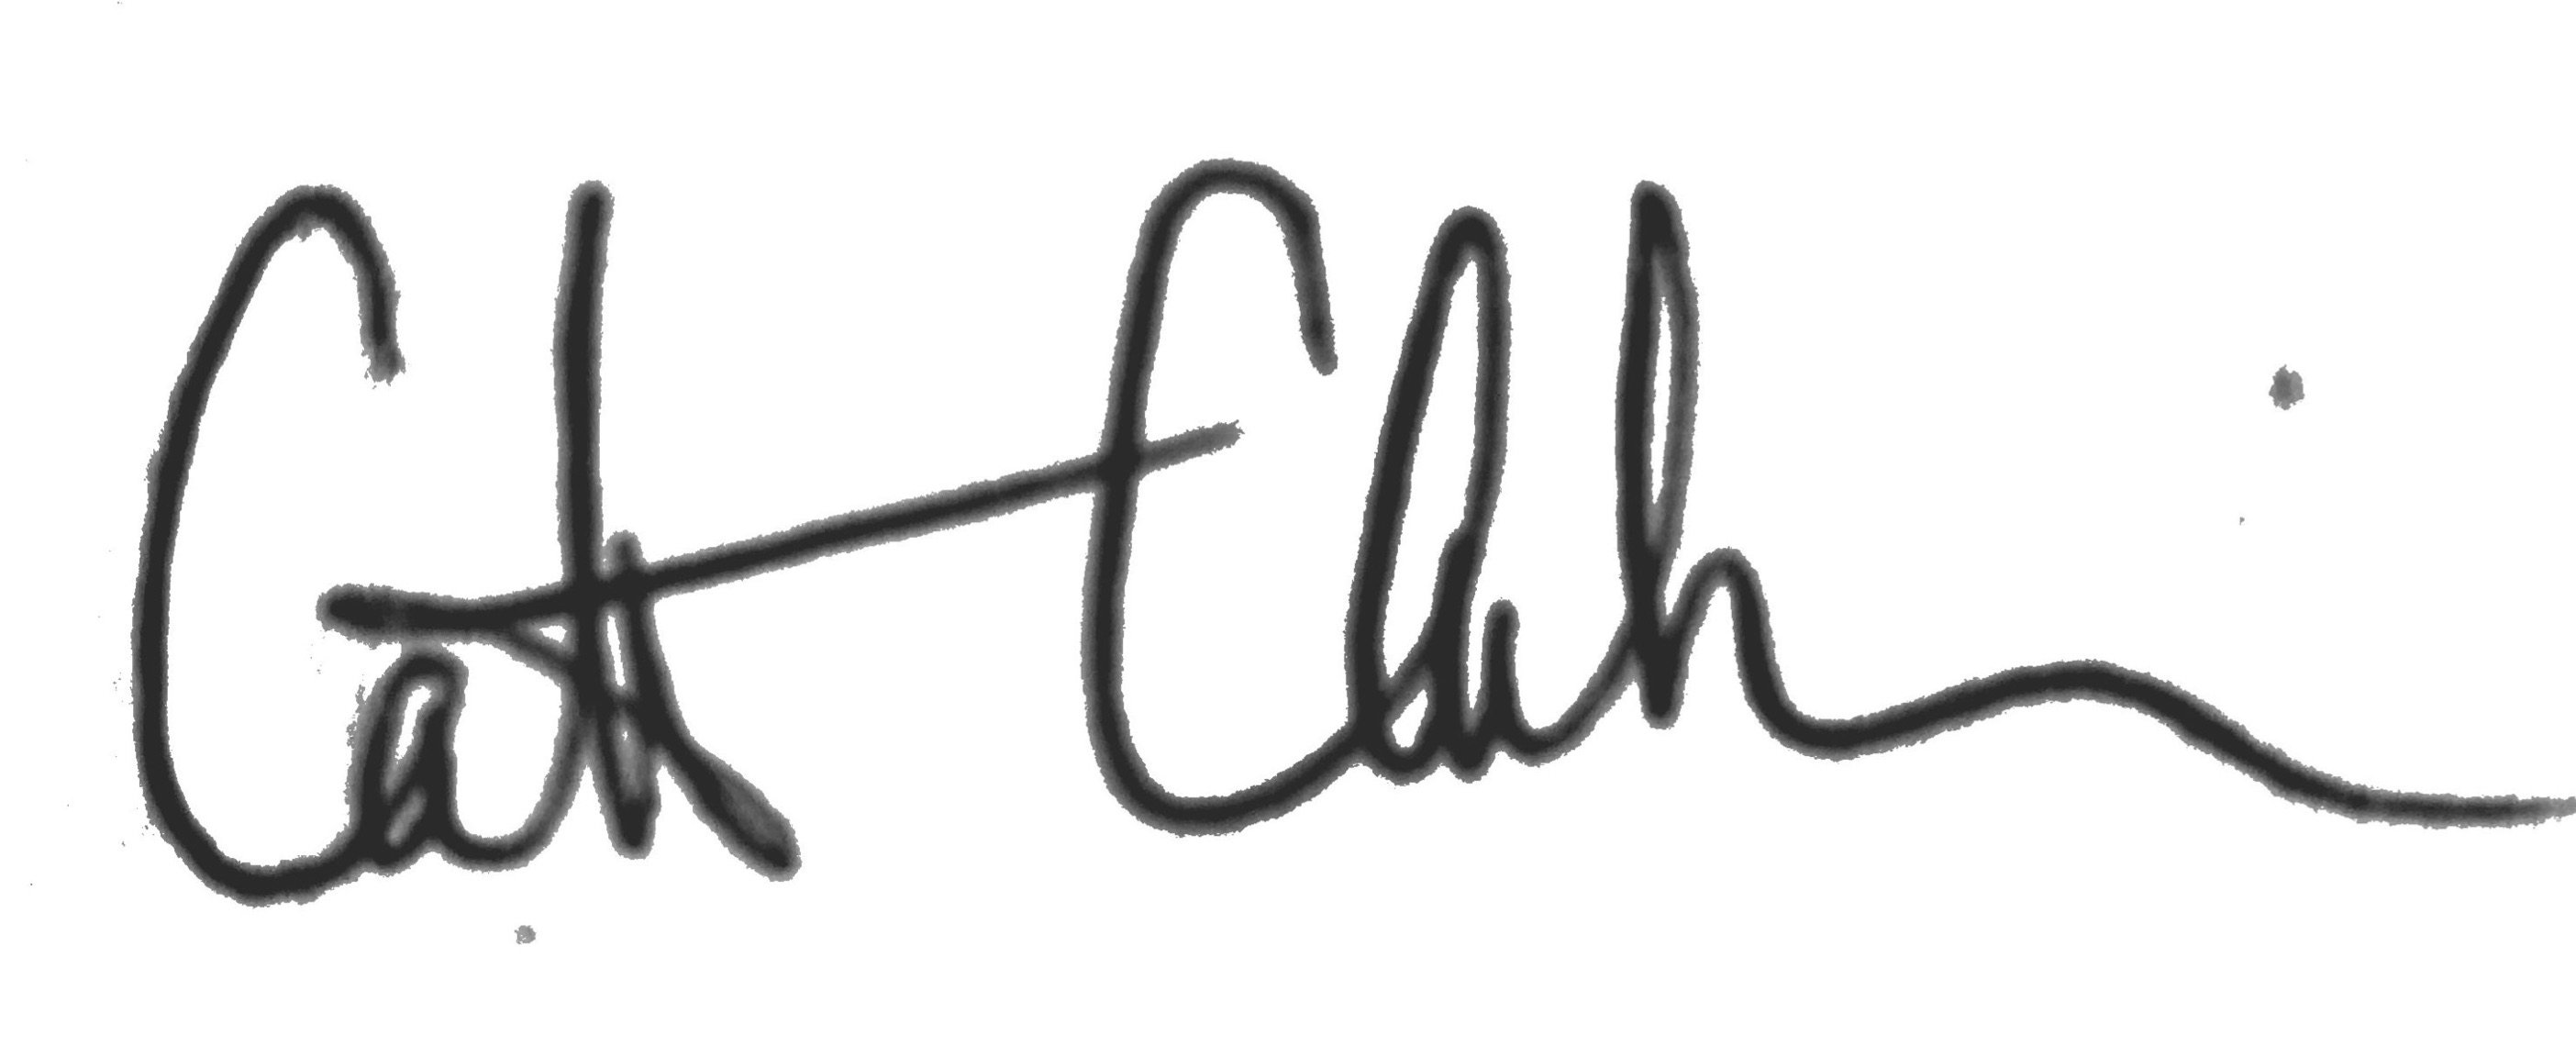
\includegraphics[width=0.2\textwidth]{Full_Signature.jpg} \\
 

\noindent Catherine J Chamberlain


\end{letter}
\end{document}
